% Options for packages loaded elsewhere
\PassOptionsToPackage{unicode}{hyperref}
\PassOptionsToPackage{hyphens}{url}
%
\documentclass[
]{article}
\usepackage{amsmath,amssymb}
\usepackage{iftex}
\ifPDFTeX
  \usepackage[T1]{fontenc}
  \usepackage[utf8]{inputenc}
  \usepackage{textcomp} % provide euro and other symbols
\else % if luatex or xetex
  \usepackage{unicode-math} % this also loads fontspec
  \defaultfontfeatures{Scale=MatchLowercase}
  \defaultfontfeatures[\rmfamily]{Ligatures=TeX,Scale=1}
\fi
\usepackage{lmodern}
\ifPDFTeX\else
  % xetex/luatex font selection
\fi
% Use upquote if available, for straight quotes in verbatim environments
\IfFileExists{upquote.sty}{\usepackage{upquote}}{}
\IfFileExists{microtype.sty}{% use microtype if available
  \usepackage[]{microtype}
  \UseMicrotypeSet[protrusion]{basicmath} % disable protrusion for tt fonts
}{}
\makeatletter
\@ifundefined{KOMAClassName}{% if non-KOMA class
  \IfFileExists{parskip.sty}{%
    \usepackage{parskip}
  }{% else
    \setlength{\parindent}{0pt}
    \setlength{\parskip}{6pt plus 2pt minus 1pt}}
}{% if KOMA class
  \KOMAoptions{parskip=half}}
\makeatother
\usepackage{xcolor}
\usepackage[margin=1in]{geometry}
\usepackage{graphicx}
\makeatletter
\def\maxwidth{\ifdim\Gin@nat@width>\linewidth\linewidth\else\Gin@nat@width\fi}
\def\maxheight{\ifdim\Gin@nat@height>\textheight\textheight\else\Gin@nat@height\fi}
\makeatother
% Scale images if necessary, so that they will not overflow the page
% margins by default, and it is still possible to overwrite the defaults
% using explicit options in \includegraphics[width, height, ...]{}
\setkeys{Gin}{width=\maxwidth,height=\maxheight,keepaspectratio}
% Set default figure placement to htbp
\makeatletter
\def\fps@figure{htbp}
\makeatother
\setlength{\emergencystretch}{3em} % prevent overfull lines
\providecommand{\tightlist}{%
  \setlength{\itemsep}{0pt}\setlength{\parskip}{0pt}}
\setcounter{secnumdepth}{-\maxdimen} % remove section numbering
\usepackage{tabularx}
\usepackage{dcolumn}
\usepackage[version=4]{mhchem}
\usepackage{pdflscape}
\newcommand{\blandscape}{\begin{landscape}}
\newcommand{\elandscape}{\end{landscape}}
\usepackage{amsmath, mhchem}
\usepackage{booktabs}
\usepackage{longtable}
\usepackage{array}
\usepackage{multirow}
\usepackage{wrapfig}
\usepackage{float}
\usepackage{colortbl}
\usepackage{pdflscape}
\usepackage{tabu}
\usepackage{threeparttable}
\usepackage{threeparttablex}
\usepackage[normalem]{ulem}
\usepackage{makecell}
\usepackage{xcolor}
\ifLuaTeX
  \usepackage{selnolig}  % disable illegal ligatures
\fi
\usepackage{bookmark}
\IfFileExists{xurl.sty}{\usepackage{xurl}}{} % add URL line breaks if available
\urlstyle{same}
\hypersetup{
  pdftitle={Exploring the multi-scale ecological consequences of stoichiometric imbalance using an agent-based modeling approach},
  hidelinks,
  pdfcreator={LaTeX via pandoc}}

\title{Exploring the multi-scale ecological consequences of
stoichiometric imbalance using an agent-based modeling approach}
\usepackage{etoolbox}
\makeatletter
\providecommand{\subtitle}[1]{% add subtitle to \maketitle
  \apptocmd{\@title}{\par {\large #1 \par}}{}{}
}
\makeatother
\subtitle{Appendix A}
\author{}
\date{\vspace{-2.5em}}

\begin{document}
\maketitle

\section{Assumptions}\label{assumptions}

(Standard DEB assumptions from Table 2.4, DEB Book 3rd Ed, apply)

\emph{Added assumptions:}

\begin{itemize}
\tightlist
\item
  Consumer is heterotrophic and cannot separately uptake inorganic
  nutrients
\item
  Consumer is either endothermic, or an ectotherm in a thermally
  homogenous environment
\item
  Carbon content is higher than nitrogen in resources within the
  environment
\item
  Assimilated products sent to the reserves all contain carbon, but
  nitrogen is only sent to one reserve, \(M_{E_N}\). This can be
  conceptualized as how amino acids are nitrogen-rich, but also contain
  significant amounts of carbon.
\item
  The N-rich reserve, \(M_{E_N}\), gets priority for carbon assimilation
\item
  Assimilation efficiency is constant (though this model could be
  modified such that assimilation efficiency depends on resource
  quality, etc).
\item
  Movement in landscape increases the organism's somatic maintenance
  costs
\item
  Though it is customary in DEB models to excrete biomass used to build
  maturity maintenance, it is stored within the consumer in this model
\item
  Stoichiometric ratios of carbon to nitrogen are represented as
  \(q_{C}^{Var}:q_{N}^{Var}\), where \(q_{C}^{Var}=1\).
\end{itemize}

\newpage

\section{Short Introduction to Synthesizing Units
(SUs)}\label{short-introduction-to-synthesizing-units-sus}

Several metabolic processes are modeled through use of Synthesizing
Units (SUs). Simply put, SUs are able to create a product with fixed
stoichiometry from streams of different flux substrates that are
comprised of different stoichiometries. SUs are analogous both
conceptually and mathematically to classical enzyme kinetics (DEBv3),
which allows us to model nutrient limitation-type dynamics. When there
is a lack of a certain substrate, the product formation (e.g., somatic
structure) is delayed. When there is excess of a certain substrate, it
is rejected, then partially recycled and the rest excreted. More details
about SUs can be found in the DEB book (Kooijman 2000) and also other
publications (Sousa et al 2010, Van der Meer 2022). Additionally, our
model uses only ``parallel'' binding, where the order of substrates
binding to the SU does not alter the kinetics of SU production.

There are 2 forms of SU production used in this model, details of which
can be found in Chapter 3 of (Kooijman 2000):

\begin{enumerate}
\def\labelenumi{\arabic{enumi}.}
\tightlist
\item
  A ``demand'' SU, which has a constant draw for substrates to meet
  production needs. These are used for meeting maintenance costs.
\item
  A ``supply'' SU, which requires all of the reactants must be in the
  appropriate amounts to create one unit of product, and will not
  turnover product until all substrates are bound. A graphical example
  of this is below.
\end{enumerate}

\begin{figure}
\centering
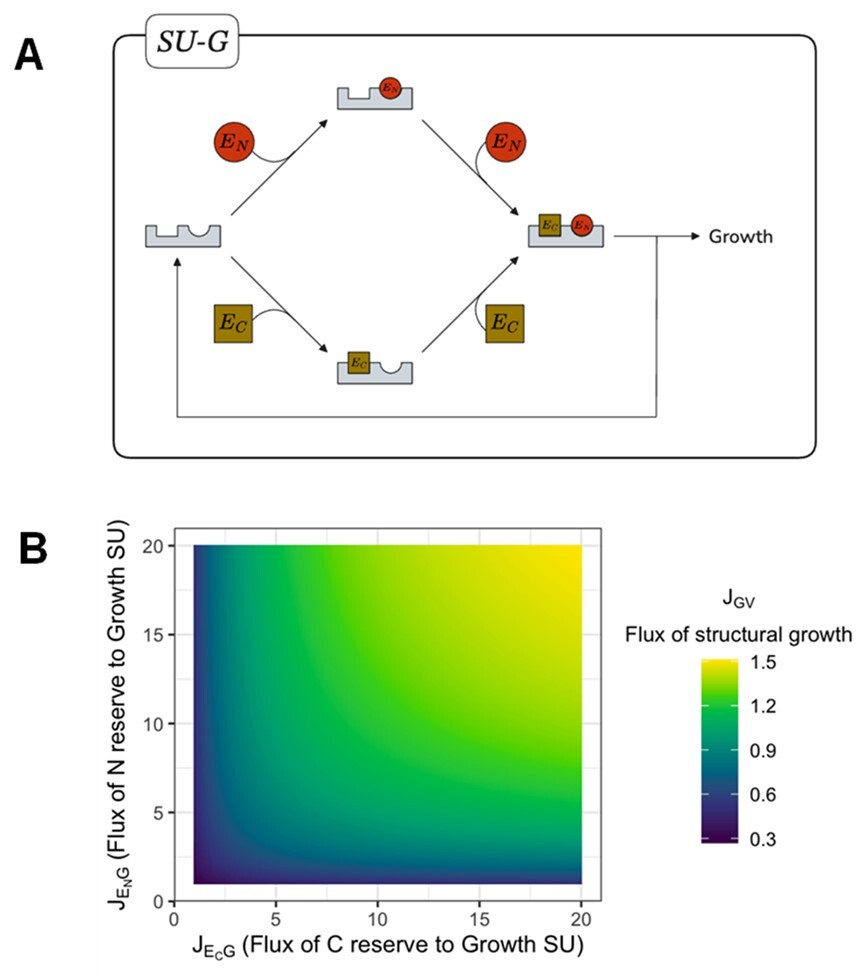
\includegraphics{SU_diagram_example.jpg}
\caption{An example of a supply Synthesizing Unit (SU), as used in the
somatic growth process. Panel A is a diagram of C-rich and N-rich
reserve combining to create a unit of somatic structure. The dynamics of
somatic growth flux are controlled by the input fluxes of the C-rich and
N-rich reserves, as seen in panel B.}
\end{figure}

\newpage

\section{Theory/Model Derivations}\label{theorymodel-derivations}

\subsubsection{Diagram of Model and Overview of Important Model
Mechanisms}\label{diagram-of-model-and-overview-of-important-model-mechanisms}

\begin{figure}
\centering
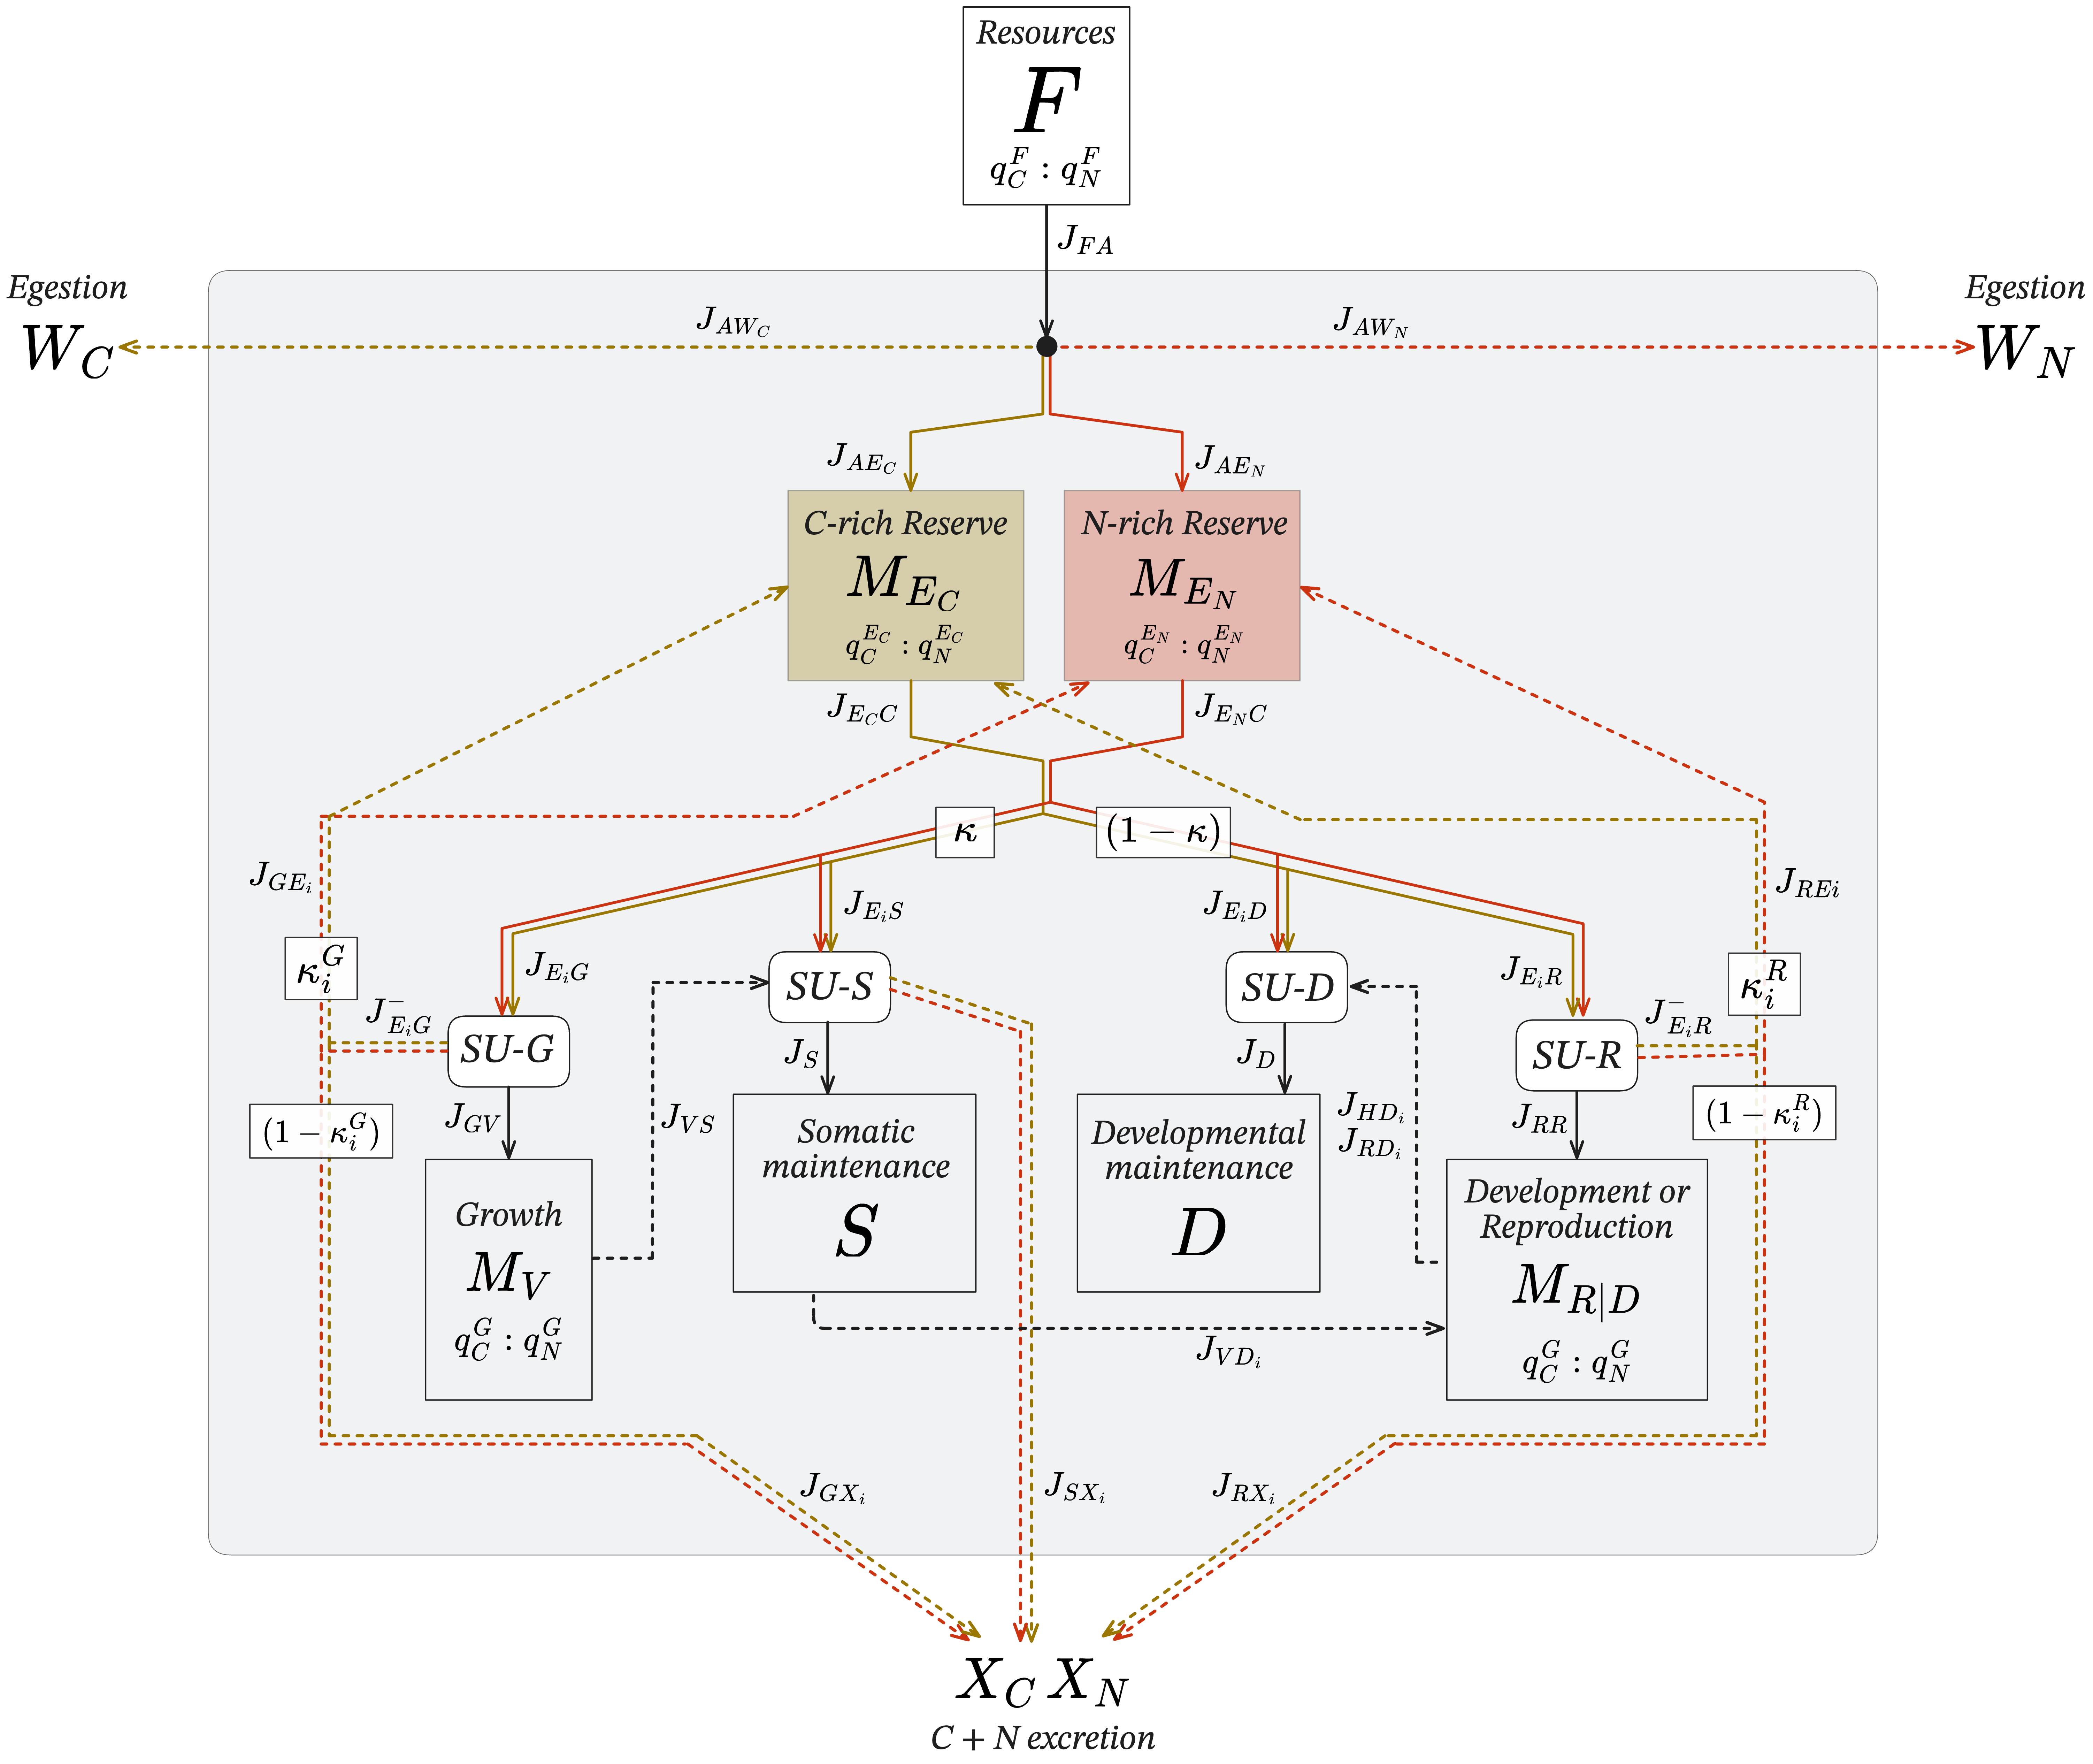
\includegraphics{woodstoich_appendixA_diagram.png}
\caption{Flow diagram of nutrient metabolism through free-living
organism}
\end{figure}

See Table 1 at the end of this document for terms.

\newpage

\section{Mass Balance Equations}\label{mass-balance-equations}

\begin{align}
\frac{dF}{dt} &= - J_{FA}
\\\nonumber
\\
\frac{d{W_{C}}}{dt} &= J_{W_C}
\\\nonumber
\\
\frac{d{W_{N}}}{dt} &= J_{W_N}
\\\nonumber
\\
\frac{d{M_{E_{C}}}}{dt} &= J_{AE_{C}} + J_{GR{E_C}} - J_{E_{C}C}
\\\nonumber
\\
\frac{d{M_{E_{N}}}}{dt} &= J_{AE_{N}} + J_{GR{E_N}} - J_{E_{N}C}
\\\nonumber
\\
\frac{dM_V}{dt} &= J_{GV} - J_{VS} - J_{VD}
\\\nonumber
\\
\frac{d{M_H}}{dt} &= 
\begin{cases}
J_{RR} & \qquad \text{if } {M_H} < M_{H}^{p} \\
0      & \qquad \text{if } {M_H} \ge M_{H}^{p} 
\end{cases}
\\\nonumber
\\
\frac{d{M_R}}{dt} &= 
\begin{cases}
0 & \qquad \text{if } {M_H} < M_{H}^{p} \\
J_{RR}      & \qquad \text{if } {M_H} \ge M_{H}^{p}  
\end{cases}
\\
\frac{d{X_C}}{dt} &= J_{{E_C}S} + J_{{E_C}D} + J_{{E_N}S} + J_{{E_N}D}+ J_{GRX{E_C}} + J_{GRX{E_N}} + J_{VS} + J_{VD}
\\
\\\nonumber
\frac{d{X_N}}{dt} &= \frac{q_{N}^{E_N}}{q_{C}^{E_N}}\biggr(J_{{E_N}S} + J_{{E_N}D} + J_{GRX{E_N}}\biggr) + \frac{q_{N}^{V}}{q_{C}^{V}}\biggr(J_{VS} + J_{VD}\biggr)
\end{align}

\newpage

\section{Flux Derivations}\label{flux-derivations}

To complete the balance equations with relevant parameters, flux terms
must be further specified.

\subsection{\texorpdfstring{Ingestion
(\(J_{FA}\))}{Ingestion (J\_\{FA\})}}\label{ingestion-j_fa}

The consumer will ingest resources (\(F\)) in terms of mol-C, with a
ratio of C:N of \(q_{C}^{F}:q_{N}^{F}\). The ingestion flux is
proportional to the surface area of the consumer, such that:

\begin{align*}
J_{FA} &= f\,{\{J_{X{A_M}}\}}\,{V^{2/3}}
\end{align*}

Where \(\{J_{X{A_M}}\}\) is the consumer surface area-specific maximum
ingestion rate, \(V\) is the consumer body volume, and \(f\) is the
Holling Type II scaled functional response.

The form of the Type II functional response used is: \begin{align}
\frac{F}{{F_H}+F}
\end{align}

Where \({F_H}\) is the half-saturation constant, which is defined as:

\begin{align*}
F_H &= \frac{\{J_{X{A_M}}\}}{\{F_M\}}
\end{align*}

Where \(\{F_M\}\) is the surface-area specific searching rate.

For this model, it is useful to define the consumer in terms of body
mass instead of volume. To define the surface-area specific ingestion
rate, we will convert consumer structural volume to biomass, \(M_V\)
(mol C), for the final form. Due to DEB theory's assumption of strong
homeostasis (biochemical composition of state variables must be
constant), we can say that the ratio of consumer biomass to volume is
constant: \([M_V] = \frac{M_V}{V}\), where \([M_V]\) is the
volume-specific structural biomass. Note that this does not mean that
\emph{overall stoichiometry} of an organism must remain fixed, as the
ratio of reserves to structure (known as \emph{reserve density},
\(m_{E_i}\)) leads to fluctuations in whole-organism stoichiometries.

For convenience, throughout the model, all internal fluxes will be in
units of (\(\frac{\text{mol C}}{t}\)). The stoichiometries of each state
variable will be used to convert between elements and total masses.
Thus, for ingestion:

\begin{align}
J_{FA} &= f\,{\{J_{X{A_M}}}\}\,{\biggl(\frac{M_V}{[M_V]}\biggr)^{2/3}}
\end{align}

\subsection{\texorpdfstring{Assimilation
(\(J_{A{E_i}}\))}{Assimilation (J\_\{A\{E\_i\}\})}}\label{assimilation-j_ae_i}

Upon entering the consumer, \(F\) will become assimilated into two
reserves: \(M_{E_C}\), the carbon-rich reserve, and \(M_{E_N}\), the
nitrogen-rich reserve. In this model, assimilation efficiencies are
constant. Carbon assimilation is prioritized to \(M_{E_N}\) before
\(M_{E_C}\).

The assimilation of resource to the N--rich reserve is:

\begin{align}
J_{A{E_N}} &= \biggl(\frac{q\strut_{N}^{F}}{q\strut_{C}^{F}}\biggr)\biggl(\frac{q\strut_{C}^{E_N}}{q\strut_{N}^{E_N}}\biggr)Y_{{E_N}F}\,J_{FA}
\end{align}

Where \(\biggl(\frac{q_{i}^{F}}{q_{C}^{F}}\biggr)\) is the molar
proportion of element-\(i\) in the resource. \({q_{C}^{E_i}}\) couples
the amount of carbon to the amount of nitrogen that will be assimilated
into reserve\(-i\). This coupling ensures that a common flux currency of
\(\biggl(\frac{mol-C}{time}\biggr)\) is used throughout the internal
consumer calculations.

To determine the amount of carbon sent to the carbon-rich reserve,
\(M_{E_C}\), we will determine how much total carbon could be
assimilated from the food, then subtract the amount of carbon sent to
\(M_{E_N}\) , which takes priority:

\begin{align}
J_{A{E_C}} &= Y_{{E_C}F}\,J_{FA} - J_{A{E_N}}
\end{align}

\subsection{\texorpdfstring{Waste/Egestion
(\(J_{W_i}\))}{Waste/Egestion (J\_\{W\_i\})}}\label{wasteegestion-j_w_i}

To calculate the amount of waste (\(W_C\) and \(W_N\)), we will simply
determine what was not assimilated from the ingested resource. Egestion
fluxes will be in terms of carbon- and nitrogen (\(\frac{mol\:C}{t}\)
and \(\frac{mol\:N}{t}\))

\begin{align}
J_{W_C} &= (1-Y_{{E_C}F})\,J_{FA}
\\
J_{W_N} &= \biggl(\frac{q\strut_{N}^{F}}{q\strut_{C}^{F}}\biggr)(1 - Y_{{E_N}F})J_{FA}
\end{align}

\newpage

\subsection{\texorpdfstring{Somatic Maintenance (\(J_{E_{i}S}\) and
\(J_{VS}\))}{Somatic Maintenance (J\_\{E\_\{i\}S\} and J\_\{VS\})}}\label{somatic-maintenance-j_e_is-and-j_vs}

This SU is a ``demand'' SU, in that the production flux is fixed by the
current needs of the organism. Somatic maintenance can be paid from any
reserve, and also can be paid from mobilizing structure if the reserves
are too low to pay maintenance. Mechanistically, this means the SU will
turn over whatever substrate is available.

The SU has four ``binding sites'': \(M_{E_C}\), \(M_{E_N}\), and
\(M_{V}\). The empty enzyme (i.e., nothing bound) waits for something to
bind. It prefers to use \(M_{E_C}\) above all other substrates, and
prefers to \emph{not} use structure above all other substrates. Thus,
the priority for substrate usage by the SU is:
\(\ce{M_{E_C} -> M_{E_N} -> M_{V}}\)

This priority set is created through two mechanisms: \((1)\) the rates
of SU turnover for each substrate are lower compared to each substrate
with a higher preference (\(M_{E_C}\) has the fastest turnover), which
allows for \((2)\) unpreferred substrates to be displaced by a preferred
substrate, if it is available. This approach to SU kinetics in DEB
theory are referred to as a ``Preference SU'' with substitutable
substrates. Short details are available on page 107 of the DEB book v4,
Section 3.7.4. Other methods for resolving these kinetics are explained
in Van der Meer et al 2022, under the heading ``Preference SU with Two
Substitutable Substrates''.

Note that excretion from this SU is created by the actual mass ``used''
in meeting somatic maintenance costs. The stoichiometry of excretion is
therefore based on the substrate(s) turned over by the SU (i.e.,
reserve-\(i\), etc).

\subsubsection{Somatic Maintenance SU Flux
Overview}\label{somatic-maintenance-su-flux-overview}

Since somatic maintenance is represented by the demand of a constant
rate (somatic maintenance rate coefficient, \(k_M\)) scaled to the
current body mass of the organism (\(M_V\)):

\begin{align*}
J_S &= k_{\scriptscriptstyle M}M_V
\end{align*}

For our model, we have added an additional term to this equation, which
incorporates a somatic maintenance penalty for consumer movement. The
more consumers move, the more their energetic costs increase:

\begin{align} 
J_S &= (k_{\scriptscriptstyle M}M_V)(1 + d\sigma) 
\end{align}

Where \(\sigma\) is the multiplicative parameter that controls how
severe of a penalty movement imposes, and \(d\) is the distance walked
by the consumer.

\(J_S\) is easy to calculate. What is more complex to calculate is how
much of each reserve or structure is used in the process of meeting
maintenance costs, \(J_{{E_i}S}\) if using reserve-\(i\), and/or
\(J_{VS}\) if mobilizing structure. We start by identifying that the
total demanded maintenance is paid from some combination of our four
substrates:

\begin{align}
J_S &= {k_M}{M_V} = J_{{E_C}S} + J_{{E_N}S} + J_{VS}
\\
J_S &= {k_M}{M_V} = {Y_{S{E_C}}}\,{k\strut^S_C}\,\frac{\theta\strut^{S*}_C}{\theta\strut^{S*}_{tot}} + {Y_{S{E_N}}}\,{k\strut^S_N}\,\frac{\theta\strut^{S*}_N}{\theta\strut^{S*}_{tot}} +  {Y_{S{V}}}\,{k\strut^S_V}\,\frac{\theta\strut^{S*}_V}{\theta\strut^{S*}_{tot}}
\end{align}

Where \(\theta\strut^{S*}_i\) is the proportion of SU in a particular
binding state (none, C, or N reserve) at equilibrium, and
\(\theta^{S*}_{tot}\) is the sum of all binding states at equilibrium
(\(\theta\strut^{S*}_o + \theta\strut^{S*}_C + \theta\strut^{S*}_N+ \theta\strut^{S*}_V\)).
Equilibrium values of these binding states depend on equations for the
kinetics of this SU.

\newpage

\subsubsection{Somatic Maintenance SU
Kinetics}\label{somatic-maintenance-su-kinetics}

Here we assume a ``Preference SU with four substitutable substrates''
following a derivation of a similar SU by Van Der Meer (2022). This
representation is equivalent to that of Kooijman (DEB3). Once bound to a
substrate, we assume the SU turns over (i.e., produces maintenance) at
substrate-specific rates, \({k\strut^S_i}\). The SU imposes preferential
use of substrates with higher \({k\strut^S_i}\). Additionally, we assume
that more preferred substrates can displace less preferred substrates
already bound to the SU without inhibition.

The kinetics of the SU are described below. \(\theta_{\text{o}}^S\)
corresponds to the proportion of SUs that have nothing bound (empty).
\({\theta\strut^{S}_{i}}\) and \({\theta\strut^{S}_{{V}}}\) correspond
to an SU bound with reserve-\(i\) or structure, respectively. The
arrival rates for reserve substrates are described by
\({\kappa_i}\,{J_{{E_i}C}}\), and the arrival flux of substrate is
described by \(J_{{VC}}\). The rates of SU turnover for each substrate
are described by \({k\strut^S_i}\) for reserve substrates and
\({k\strut^S_V}\) for structure.

The differential equations for the SU binding states are:

\begin{align}
\frac{d{\theta\strut^{S}_{o}}}{dt} &= {k\strut^S_C}{\theta\strut^{S}_{{C}}} + {k\strut^S_N}{\theta\strut^{S}_{{N}}} + {k\strut^S_V}{\theta\strut^{S}_{{V}}} - {\theta\strut^{S}_{o}}\biggl({\kappa_C}{J_{{E_C}C}} + {\kappa_N}{J_{{E_N}C}} + J_{{VC}}\biggr)
\\
\frac{d{\theta\strut^{S}_C}}{dt} &= {\kappa_C}\,{J_{{E_C}C}}\biggl({\theta\strut^{S}_{o}} + {\theta\strut^{S}_{N}}  + {\theta\strut^{S}_{V}}\biggr) - {k\strut^S_C}{\theta\strut^{S}_{{C}}}
\\
\frac{d{\theta\strut^{S}_N}}{dt} &= {\kappa_N}\,{J_{{E_N}C}}\biggl({\theta\strut^{S}_{o}} + {\theta\strut^{S}_{V}}\biggr) - {\theta\strut^{S}_{{N}}}\biggl({k\strut^S_N} + {\kappa_C}\,{J_{{E_C}C}}\biggr)
\\
\frac{d{\theta\strut^{S}_V}}{dt} &= J_{{VC}}{\theta\strut^{S}_{o}} - {\theta\strut^{S}_{{V}}}\biggl({k\strut^S_V} +  {\kappa_C}\,{J_{{E_C}C}} + {\kappa_N}\,{J_{{E_N}C}}\biggr)
\\
1 &= {\theta\strut^{S}_{\text{tot}}} = {\theta\strut^{S}_{o}} + {\theta\strut^{S}_{{C}}} + {\theta\strut^{S}_{N}} + {\theta\strut^{S}_{V}}
\end{align}

The steady state equations of binding states that turnover the SU are as
follows, per Mathematica (Some terms are presented as \(A\), etc, to
ensure equations fit on one line):

\begin{align}
\frac{\theta^{S*}_C}{\theta^{S*}_{tot}} &= \frac{{\kappa_C}\,{J_{{E_C}C}}}{\biggl({\kappa_C}\,{J_{{E_C}C}} + {k\strut^S_C}\biggr)}
\\
\frac{\theta^{S*}_N}{\theta^{S*}_{tot}}&= \frac{{\kappa_N}\,{J_{{E_N}C}}\,{k\strut^S_C}}{\biggl({\kappa_C}\,{J_{{E_C}C}} + {k\strut^S_C}\biggr)\biggl({\kappa_C}\,{J_{{E_C}C}} + {\kappa_N}\,{J_{{E_N}C}} + {k\strut^S_N}\biggr)}
\\
\frac{\theta^{S*}_V}{\theta^{S*}_{tot}}&= \frac{J_{{VCS}}{k\strut^S_C}\biggl({\kappa_C}\,{J_{{E_C}C}} + {k\strut^S_N}\biggr)}{\biggl({\kappa_C}\,{J_{{E_C}C}} + {k\strut^S_C}\biggr)\biggl({\kappa_C}\,{J_{{E_C}C}} + {\kappa_N}\,{J_{{E_N}C}} + {k\strut^S_N}\biggr)\biggl({\kappa_C}\,{J_{{E_C}C}} + {\kappa_N}\,{J_{{E_N}C}} + J_{VC} + {k\strut^S_V}\biggr)}
\end{align}

Note that the steady state for turning over the SU with \(M_{E_C}\) is
independent of other substrate dynamics (and mimics Michaelis-Menten
kinetics or the Holling Type II functional response). This makes sense,
given that our mechanistic goal was that if \(M_{E_C}\) is present in
enough capacity, it will turn the SU over, regardless of the presence of
\(M_{E_N}\).

As previously discussed, we can then write the turnover rate of our
unpreferred substrates as fraction of our preferred substrate, with
\(\rho\strut^S_i\) as the fractional preference parameter (e.g.,
\(\rho\strut^S_N = \frac{k^S_N}{k^S_C}\)). We then have:

\begin{align}
{k\strut^S_C} &= k_S
\\
{k\strut^S_N} &= {\rho\strut^S_N}{k_S}
\\
{k\strut^S_V} &= {\rho\strut^S_V}{k_S}
\\
1 &> {\rho\strut^S_N} > {\rho\strut^S_V}
\end{align}

If we implement the above simplification, then the steady state
equations become:

\begin{align}
\frac{\theta^{S*}_C}{\theta^{S*}_{tot}} &= \frac{{\kappa_C}\,{J_{{E_C}C}}}{\biggl({\kappa_C}\,{J_{{E_C}C}} + {k_S}\biggr)}
\\
\frac{\theta^{S*}_N}{\theta^{S*}_{tot}}&= \frac{{\kappa_N}\,{J_{{E_N}C}}\,{k_S}}{\biggl({\kappa_C}\,{J_{{E_C}C}} + {k_S}\biggr)\biggl({\kappa_C}\,{J_{{E_C}C}} + {\kappa_N}\,{J_{{E_N}C}} + {\rho\strut^S_N}{k_S}\biggr)}
\\
\frac{\theta^{S*}_V}{\theta^{S*}_{tot}}&= \frac{{J_{VCS}}{k_S}\biggl({\kappa_C}\,{J_{{E_C}C}} + {\rho\strut^S_N}{k_S}\biggr)}{\biggl({\kappa_C}\,{J_{{E_C}C}} + {k_S}\biggr)\biggl({\kappa_C}\,{J_{{E_C}C}} + {\kappa_N}\,{J_{{E_N}C}} + {\rho\strut^S_N}{k_S}\biggr)\biggl({\kappa_C}\,{J_{{E_C}C}} + {\kappa_N}\,{J_{{E_N}C}} + {J_{VCS}} + {\rho\strut^S_V}{k_S}\biggr)}
\end{align}

Additionally, the equation to meet somatic maintenance, using the
preference simplification is:

\begin{align}
J_S &= {k_M}{M_V} = k_S\,\frac{\theta\strut^{S*}_C}{\theta\strut^{S*}_{tot}} \,+\, k_S\,\rho\strut^S_N\,\frac{\theta\strut^{S*}_N}{\theta\strut^{S*}_{tot}} \,+\, \,k_S\,\rho\strut^S_V\,\frac{\theta\strut^{S*}_V}{\theta\strut^{S*}_{tot}}
\end{align}

If we additionally assume (following similarly to Van der Meer 2022) (1)
that we mobilize just as much C-mol of structure as may be needed to pay
maintenance costs if it needed to be paid by structure in full
(\(J_{VC} = J_S\))

Then it follows that: \begin{align}
J_{{E_C}S} &= \,k_S\,\frac{\theta^{S*}_C}{\theta^{S*}_{tot}} 
\\
J_{{E_N}S} &= \,k_S\,\rho\strut^S_N\,\frac{\theta^{S*}_N}{\theta^{S*}_{tot}}
\\
J_{VS} &= \,k_S\,\rho\strut^S_V\,\frac{\theta^{S*}_V}{\theta^{S*}_{tot}}
\end{align}

To solve for these four fluxes, after substituting the
\(\frac{\theta^{S*}_i}{\theta^{S*}_{tot}}\) terms, we still must define
\(k_S\). Per Eqn. \((11)\), we can see that \(k_S\) is not a free
parameter, but has a solution that can be numerically solved (Note that
if only two substrates are used for this type of SU, there is an
explicit solution for \(k_S\) using the positive root of the quadratic
formula).

Note that any mobilized structure that is not used for maintenance is
shuttled directly back to structure, so that the only dissapation of
structure is \(J_{VS}\).

\subsubsection{Somatic Maintenance
Excretion}\label{somatic-maintenance-excretion}

The dissipation of mass used in meeting maintenance costs is equal to
the cost themselves (the energy is used for the organism but the mass
itself is excreted).

\newpage

\subsection{\texorpdfstring{Developmental Maintenance
(\(J_{E_{i}D}\))}{Developmental Maintenance (J\_\{E\_\{i\}D\})}}\label{developmental-maintenance-j_e_id}

Developmental maintenance is paid through an SU (\(SU-D\)) that is
nearly identical to the somatic maintenance SU. Developmental
maintenance must be paid according to:

\begin{align}
J_D &= k_{\scriptscriptstyle J}M_H
\end{align}

Where \(k_{\scriptscriptstyle J}\) is the maturity maintenance rate
coefficient, and \(M_H\) is the current level of maturity of the
consumer.

\emph{Important note about insufficient reserves and rejuvenation}:
Unlike the somatic maintenance SU, if reserves are too low to pay
somatic maintenance, then the consumer can ``rejuvenate'', and loses its
maturity level. This comes from pg 134 of Bas Kooijman's comments on
DEBv3, seen here:
\url{https://www.bio.vu.nl/thb/deb/deblab/bib/Kooy2010_c.pdf} However,
in this model, we decided to implement that structure can also be broken
down to meet reproductive needs. This was decided both due to efficiency
in numerical solving methods in the simulation, and because we wanted to
maintain the hare precocial trait in our case study.

Since a preference SU has already been instituted, the developmental SU
therefore has substrates \(M_{E_C}\), \(M_{E_N}\), and \(M_{V}\) from
highest to lowest preference.

Following the previous steps outlined for somatic maintenance, we can
arrive at the following final fluxes: \begin{align}
\frac{\theta^{D*}_C}{\theta^{D*}_{tot}} &= \frac{(1 - {\kappa_C}){J_{{E_C}C}}}{\biggl((1 - {\kappa_C}){J_{{E_C}C}} + {k_D}\biggr)}
\\
\frac{\theta^{D*}_N}{\theta^{D*}_{tot}}&= \frac{(1 - {\kappa_N}){J_{{E_N}C}}\,{k_D}}{\biggl((1 - {\kappa_C}){J_{{E_C}C}} + {k_D}\biggr)\biggl({(1 - {\kappa_C}){J_{{E_C}C}} + (1 - {\kappa_N}){J_{{E_N}C}} + {\rho\strut^D_N}{k_D}\biggr)}}
\\
\frac{\theta^{D*}_V}{\theta^{D*}_{tot}}&= \frac{{J_{VCD}}{k_D}\biggl((1 - {\kappa_C}){J_{{E_C}C}} + {\rho\strut^D_N}{k_D}\biggr)}{A * B * C}
\\\nonumber
A &= \biggl((1 - {\kappa_C}){J_{{E_C}C}} + {k_D}\biggr)
\\\nonumber
B &= \biggl((1 - {\kappa_C}){J_{{E_C}C}} + (1 - {\kappa_N}){J_{{E_N}C}} + {\rho\strut^D_N}{k_D}\biggr)
\\\nonumber
C &= \biggl((1 - {\kappa_C}){J_{{E_C}C}} + (1 - {\kappa_N}){J_{{E_N}C}} + {J_{VCD}} + {\rho\strut^D_V}{k_D}\biggr)
\\
J_{{E_C}D} &= \,k_D\,\frac{\theta^{D*}_C}{\theta^{D*}_{tot}} 
\\
J_{{E_N}D} &= \,k_D\,\rho\strut^D_N\,\frac{\theta^{D*}_N}{\theta^{D*}_{tot}}
\\
J_{VD} &= \,k_D\,\rho\strut^D_V\,\frac{\theta^{D*}_V}{\theta^{D*}_{tot}}
\end{align}

Note that numerical solving is also needed for these fluxes.

Similar to somatic growth, all mass used in meeting development
maintenance costs is excreted into the environment.

\newpage

\subsection{\texorpdfstring{Somatic Growth (\(J_{GV}\) and
\(J_{E_{i}G}\))}{Somatic Growth (J\_\{GV\} and J\_\{E\_\{i\}G\})}}\label{somatic-growth-j_gv-and-j_e_ig}

Somatic growth occurs when 1) somatic maintenance costs are met and 2)
enough of \emph{n}-nutrients are in reserves to create a unit of
structural mass. Structure is assumed to have fixed stoichiometry.
\(J_{GV}\) is the flux of structural growth, produced by the growth SU,
\(SU\)-\(G\).

\(J_{E_{i}G}\) is the flux from reserve-\emph{i} to the growth SU,
\(SU\)-\(G\), as specified by: \begin{align}
J_{E_{i}G} &= {\kappa_{i}} J_{E_{i}C}-J_{E_{i}S}
\end{align}

Where \({\kappa_{i}}\) is the portion of flux mobilized from
reserve-\emph{i} (\(J_{E_{i}C}\)) that goes towards somatic growth and
maintenance, following Kooijman's \(\kappa\)-rule, \(J_{E_{i}S}\) is the
flux from reserve-\emph{i} to somatic maintenance.

\subsubsection{Growth SU Kinetics}\label{growth-su-kinetics}

We represent this as a parallel, complementary SU (substrate \(A\)
binding is not dependent on substrate \(B\) being bound first), more
details can be found on pg. 105 of DEBv3. Material from all three
reserves can bind in any order, but a unit of structure is not formed
until enough of reserves \(-C\) and \(-N\) are bound to the SU. Reserve
fluxes in excess are rejected by the SU \(J_{E_{i}G}^{-}\), with some
portion \(\kappa_{i}^{G}\) recycled back into the reserves and
\(\biggl(1-\kappa_{i}^{G}\biggr)\) is excreted into the environment

The kinetics of the growth SU (\(SU-G\)) are given below.
\(\theta_{\text{o}}^G\) corresponds to the density of SUs that have
nothing bound (empty). \(\theta_{CN}^G\) corresponds to the SU bound
with all three reserves. There is no difference in binding probability
in substrate binding order (\(M_{E_C}\) will bind with the same affinity
if the SU empty or has \(M_{E_N}\) bound already).

The full ODE set of SU kinetics are given as:

\begin{align}
\frac{d\theta\strut_{\text{o}}^G}{dt} &= k_{\scriptscriptstyle G}\theta\strut_{\text{CN}}^{G} - \theta\strut_{\text{o}}^G\biggl(\frac{J_{E_{C}G}}{Y_{{E_C}V}} + \frac{J_{E_{N}G}}{Y_{{E_N}V}}\biggr)
\\
\frac{d\theta\strut_{\text{C}}^G}{dt} &= {\theta\strut_{\text{o}}^G}\frac{J_{E_{C}G}}{Y_{{E_C}V}} - {\theta\strut_{\text{C}}^G}\frac{J_{E_{N}G}}{Y_{{E_N}V}}
\\
\frac{d\theta\strut_{\text{N}}^G}{dt} &= {\theta\strut_{\text{o}}^G}\frac{J_{E_{N}G}}{Y_{{E_N}V}} - {\theta\strut_{\text{C}}^G}\frac{J_{E_{C}G}}{Y_{{E_C}V}}
\\
\frac{d\theta\strut_{\text{CN}}^G}{dt} &= {\theta\strut_{\text{N}}^G}\frac{J_{E_{C}G}}{Y_{{E_C}V}} + {\theta_{\text{C}}^G}\frac{J_{E_{N}G}}{Y_{{E_N}V}} - k_{\scriptscriptstyle G}\theta\strut_{\text{CN}}^{G}
\end{align}

Where \(Y_{{E_i}V}\) is the yield of reserve on structure (i.e., how
many units of reserve \(M_{E_i}\) are needed to make one unit of
structure)

\subsubsection{Growth SU Fluxes}\label{growth-su-fluxes}

The reaction occurs when units of \(M_{E_C}\), and \(M_{E_N}\) are bound
to the SU (SU state \(\theta\strut_{\text{CN}}^G\)) and the SU
disassociates at rate \(k_{\scriptscriptstyle G}\). Therefore, the flux
of somatic growth is:

\begin{align}
J_{GV} &= k_{\scriptscriptstyle G}\theta\strut_{\text{CN}}^{G\text{*}} 
\end{align}

Where \(\theta_{\text{CN}}^{G\text{*}}\) is the steady state of the
fully bound SU. Using Mathematica or Kooijman 1998 (\emph{Biophys Chem})
Equation 10, to solve for \(\theta\strut_{\text{CNP}}^{G\text{*}}\), the
fully specified somatic growth flux is:

\begin{align}
  J_{GV} &= \biggl(\biggl(\frac{J_{E_{C}G}}{Y_{{E_C}V}}\biggr)^{-1} + \biggl(\frac{J_{E_{N}G}}{Y_{{E_N}V}}\biggr)^{-1} - \biggl(\frac{J_{E_{C}G}}{Y_{{E_C}V}} + \frac{J_{E_{N}G}}{Y_{{E_N}V}}\biggr)^{-1}\biggr)^{-1}
\end{align}

\subsubsection{Stoichiometry of Somatic
Structure}\label{stoichiometry-of-somatic-structure}

The yield parameters, \(Y_{{E_i}V}\), are defined by the stoichiometries
measured by the user.

It may be more intuitive to think of these yield parameters as the
number of substrates that must bind to the SU to form the reaction. To
make one unit (mole) of structure from reserves, we must conceptualize
how many C-mol and N-mol are being bound and combined at the SU. The
mols of each reserve that binds to the growth SU (\(n_{E_i}^{V}\)) to
produce some amount of structure (\(n_V\)) follow:

\begin{align}
{q\strut_{C}^{V}}{n_V} &= {q\strut_{C}^{E_C}}{n_{E_C}^{V}} + {q\strut_{C}^{E_N}}{n_{E_N}^{V}}
\\
{q\strut_{N}^{V}}{n_V} &= {q\strut_{N}^{E_C}}{n_{E_C}^{V}} + {q\strut_{N}^{E_N}}{n_{E_N}^{V}}
\end{align}

To convert between mol C of the state variables, the yields must follow
:

\begin{align}
Y_{{E_C}V} &= \frac{{n_{E_C}^{V}}{q\strut_{C}^{E_C}}}{{n_V}{q\strut_{C}^{V}}}
\\
Y_{{E_N}V} &= \frac{{n_{E_N}^{V}}{q\strut_{C}^{E_N}}}{{n_V}{q\strut_{C}^{V}}}
\end{align}

and \(n_V = 1\)

\subsubsection{Other Important Fluxes from Growth
SU}\label{other-important-fluxes-from-growth-su}

To track reserve recycling and environmental dissipation (i.e.,
excretion) from rejected SU fluxes, the following relationships are
needed:

The input to the SU, \(J_{E_{i}G}\), is split into two fluxes: that
which is accepted (bound) to the SU, \(J_{E_{i}G}^{+}\), and that which
is rejected (excess), \(J_{E_{i}G}^{-}\), . The obvious quantity then:

\begin{equation}
J_{E_{i}G} = J_{E_{i}G}^{+} + J_{E_{i}G}^{-}
\end{equation}

\begin{align}
J_{E_{i}G}^{+} &= {J_{GV}}{Y_{{E_i}V}}
\\
J_{E_{i}G}^{-} &= J_{{E_i}G} - J_{E_{i}G}^{+}
\\
J_{G{X{_C}}} &= \biggl(1-\kappa_{C}^{G}\biggr)J_{E_{C}G}^{-} + \biggl(1-\kappa_{N}^{G}\biggr)J_{E_{N}G}^{-}
\\
J_{G{X{_N}}} &= \frac{q^{E_N}_N}{q^{E_N}_C}\biggl(1-\kappa_{N}^{G}\biggr)J_{E_{N}G}^{-}
\end{align}

\newpage

\subsection{\texorpdfstring{Reproduction and Development (\(J_{RR}\) and
\(J_{E_{i}R}\))}{Reproduction and Development (J\_\{RR\} and J\_\{E\_\{i\}R\})}}\label{reproduction-and-development-j_rr-and-j_e_ir}

Reproduction and development (i.e., maturity) come from the reproduction
SU, \(SU-R\), in a similar design as structural growth from \(SU-G\).
However, an organism will develop (i.e., mature) until a certain
threshold when it is then able to begin reproducing, \(D_R\), as seen in
Eqs \((7)\) and \((8)\).

\(J_{E_{i}R}\) is the flux from reserve-\emph{i} to the reproduction SU,
\(SU-R\), as specified by: \begin{equation}
J_{E_{i}R}=(1-{\kappa\strut_{i}}) J_{E_{i}C}-J_{E_{i}D}
\end{equation}

Following the same derivation as in the structural growth SU, we arrive
at the following equation:

\begin{align}
  J_{RR} &= \biggl(\biggl(\frac{J_{E_{C}R}}{Y_{{E_C}R}}\biggr)^{-1} + \biggl(\frac{J_{E_{N}R}}{Y_{{E_N}R}}\biggr)^{-1} - \biggl(\frac{J_{E_{C}R}}{Y_{{E_C}R}} + \frac{J_{E_{N}R}}{Y_{{E_N}R}}\biggr)^{-1}
\end{align}

Additional fluxes of interest are derived via the same method as
outlined in the somatic growth SU section:

\begin{align}
J_{E_{i}R}^{+} &= {J_{RR}}{Y_{{E_i}R}}
\\
J_{E_{i}R}^{-} &= J_{{E_i}R} - J_{E_{i}R}^{+}
\\
J_{R{X{_C}}} &= \biggl(1-\kappa_{C}^{R}\biggr)J_{E_{C}R}^{-} + \biggl(1-\kappa_{N}^{R}\biggr)J_{E_{N}R}^{-}
\\
J_{R{X{_N}}} &= \frac{q^{E_N}_N}{q^{E_N}_C}\biggl(1-\kappa_{N}^{R}\biggr)J_{E_{N}R}^{-}
\end{align}

The organism will use \(J_{RR}\) to mature/develop reproductively
(\(M_H\)), until they reach a threshold, \(M_{H}^{p}\), at which point
they are no longer a juvenile and can reproduce. Following this
threshold, they maintain \(M_H = M_{H}^{p}\), and instead build their
reproductive buffer, \(M_R\) with \(J_{RR}\). Once their reproductive
buffer is full enough to produce offspring, \(M_{R}^{b}\), they will
reproduce, and their reproductive buffer will reset to 0.

\newpage

\subsection{Excretion Dynamics}\label{excretion-dynamics}

To account for total excretion from the organism, we will simply gather
all fluxes of excretion from each of the SUs. We have ensured that we
have converted reserves to mol-element when needed (i.e., detailing the
mol-N from excreted rejected reserve from the growth SU). Note that the
\(\kappa_{i}^{Var}\) parameters below are the fraction of rejected SU
flux that are recycled back to the reserves, and
\((1- \kappa_{i}^{Var})\) are excreted into the environment. This
ensures that the reserves do not fill above their maximum (Kooijman
2000).

The combined fluxes of rejected reserves from \(SU-G\) and \(SU-R\) that
are recycled back to their reserves are: \begin{align}
J_{GR{E_C}} &= \kappa_{C}^{G}J_{E_{C}G}^{-} + \kappa_{C}^{R}J_{E_{C}R}^{-}
\\
J_{GR{E_N}} &= \kappa_{N}^{G}J_{E_{N}G}^{-} + {\kappa_{N}^{R}}J_{E_{N}R}^{-} 
\end{align}

And the combined fluxes of rejected reserves from \(SU-G\) and \(SU-R\)
that are excreted into the environment are: \begin{align}
J_{GR{X_{E_C}}} &= \biggl(1-\kappa_{C}^{G}\biggr)J_{E_{C}G}^{-} + \biggl(1-\kappa_{C}^{R}\biggr)J_{E_{C}R}^{-}
\\
J_{GR{X_{E_N}}} &= \biggl(1-\kappa_{N}^{G}\biggr)J_{E_{N}G}^{-} + \biggl(1-\kappa_{N}^{R}\biggr)J_{E_{N}R}^{-}
\end{align}

\newpage

\subsection{\texorpdfstring{Reserve Dynamics
(\(J_{E_{i}C}\))}{Reserve Dynamics (J\_\{E\_\{i\}C\})}}\label{reserve-dynamics-j_e_ic}

We have one last flux to derive, the reserve mobilization flux,
\(J_{E_{i}C}\). The reserve dynamics are the heart of DEB theory,
buffering organisms from short-term nutrient limitation. For reference,
it is recommended to visit the strong and weak homeostasis DEB
assumptions for building intuition about how this will be derived.

While we can deduce that the reserve mobilization flux must be:

\begin{align*}
J_{{E_i}C} &= J_{{E_i}S} + J_{{E_i}D} + J_{{E_i}G} + J_{{E_i}R}
\end{align*}

However, this form isn't informative, as those fluxes are defined by
\(J_{{E_i}C}\).

We can get another form of \(J_{{E_i}C}\) from discussing a quantity
that is often helpful: reserve density, \(\varepsilon=\frac{E}{V}\) or
\(m_E = \frac{M_E}{M_V}\), depending on the formulation most convenient.
Here, we will use \(m_E\).

Reserve density acts as a physiological indicator of nutritional status:
when it is high, it indicates that the consumer has a high level of
reserve storage. As it approaches 0, the organism is starving, as very
little of its total bodymass is any nutrient storage.

To begin, we can simply make a mass-balance equation of reserve density.
There are numerous ways to do this, but we will take the following
approach:

If \(m_{E_i} = \frac{M_{E_i}}{M_V}\), and we have already built
\(\frac{d{M_{E_i}}}{dt}\) and \(\frac{d{M_V}}{dt}\) from mass-balance,
then to determine \(\frac{d{m_{E_i}}}{dt}\), we can use the calculus
quotient rule to derive:

\begin{align*}
\frac{d{m_{E_i}}}{dt} &= \frac{1}{M_V}\biggr(\frac{d{M_{E_i}}}{dt} - \frac{M_{E_i}}{M_V}\frac{dM_V}{dt}\biggr)
\\
&= \frac{1}{M_V}\biggl(\frac{dM_{E_i}}{dt}\biggr) - m_{E_i}\dot{r}
\\
\end{align*}

Where \(\dot{r}\) is the specific growth rate parameter, defined in DEB
theory as \(\dot{r}=\frac{1}{M_V}\frac{dM_V}{dt}\). Additionally, the
term \(-m_{E_i}\dot{r}\) accounts for ``reserve dilution by growth'' (as
consumer grows with same amount of reserve, the reserve density will
decrease)

This brings us to one of two important forms of the dynamics of reserve
density:

\begin{align}
\frac{d{m_{E_i}}}{dt} &= \frac{1}{M_V}\biggl(J_{AE_{i}} + J_{GR{E_i}} - J_{E_{i}C}\biggr) - m_{E_i}\dot{r}
\end{align}

Another form is drawn from the weak homeostasis assumption, and can be
read in more depth in Ch2 of DEB book v3. The equation, modified from
DEBv3 \((\text{Eq. }3.8)\) is:

\begin{align}
\frac{dm_{E_i}}{dt} &= \frac{\{J_{{A{E_i}}_M}\}}{M_V}\biggl(f - \frac{m_{E_i}}{m_{{E_i}_M}}\biggr) + \frac{J_{GR{E_i}}}{M_V}
\end{align}

Where \(\{J_{{A{E_i}}_M}\}\) is the surface-area specific maximum
assimilation flux to reserve\(-i\). This can be calculated from
\(\frac{J_{A{E_i}}}{V^2}\), where \(f=1\):
\(\{J_{{A{E_N}}_M}\}=\{J_{X{A_M}}\}Y_{F{E_N}}q\strut_{C}^{E_N}\biggl(\frac{q\strut_{N}^{F}}{q\strut_{C}^{F} + q\strut_{N}^{F}}\biggr)\)
and
\(\{J_{{A{E_C}}_M}\}=\{J_{X{A_M}}\}Y_{F{E_C}}\biggl(\frac{q\strut_{C}^{F}}{q\strut_{C}^{F} + q\strut_{N}^{F}}\biggr)-\{J_{{A{E_N}}_M}\}\)

If we isolate \(J_{{E_i}C}\) from
\(\frac{dm_{E_i}}{dt}=\frac{dm_{E_i}}{dt}\), then you can arrive at:

\begin{align}
J_{{E_i}C} &= m_{E_i}\biggl(\frac{\{J_{{A{E_i}}_M}\}}{m_{{E_i}_M}} - {M_V}\dot{r}\biggr)
\end{align}

Where \(m_{{E_i}_M}\) is the maximum reserve\(-i\) density.

A version with compound parameters (avoids mis-estimating dependent
parameters) is found through conversions using page 93 and the Appendix
of DEBv3 book, and seen in Sousa et al 2010, \(Eq.\;3\):

\begin{align}
J_{{E_i}C} &= {M_{E_i}}\biggl(\dot{\nu}\biggl(\frac{M_V}{[M_V]}\biggr)^{-1/3} - \dot{r}\biggr)
\end{align}

\newpage

\section{Table 1: Definitions of
Terms}\label{table-1-definitions-of-terms}

\renewcommand{\arraystretch}{1.15}
\begin{table}[!h]
\centering
\begin{tabular}{>{\centering\arraybackslash}m{1.5cm}>{\raggedright\arraybackslash}m{12cm}>{\centering\arraybackslash}m{2.5cm}}
\toprule
\multicolumn{1}{>{\centering\arraybackslash}p{1.5cm}}{\begingroup\fontsize{11}{13}\selectfont Term\endgroup} & \multicolumn{1}{>{\centering\arraybackslash}p{12cm}}{\begingroup\fontsize{11}{13}\selectfont Description\endgroup} & \multicolumn{1}{>{\centering\arraybackslash}p{2.5cm}}{\begingroup\fontsize{11}{13}\selectfont Units\endgroup}\\
\midrule
\addlinespace[0.3em]
\multicolumn{3}{l}{\textbf{State Variables}}\\
\cellcolor{gray!10}{\hspace{1em}$F$} & \cellcolor{gray!10}{Resource} & \cellcolor{gray!10}{mol C}\\
\hspace{1em}$M_{E_i}$ & Reserve$-i$ biomass & mol C\\
\cellcolor{gray!10}{\hspace{1em}$E_i$} & \cellcolor{gray!10}{Reserve$-i$ energy} & \cellcolor{gray!10}{$J$}\\
\hspace{1em}$m_{E_i}$ & Reserve$-i$ density $\biggl(\frac{M_{E_i}}{M_V}\biggr)$ & $(\text{mol C})(\text{mol C})^{-1}$\\
\cellcolor{gray!10}{\hspace{1em}$M_V$} & \cellcolor{gray!10}{Somatic structural biomass} & \cellcolor{gray!10}{mol C}\\
\hspace{1em}$L$ & Somatic structural length & cm\\
\cellcolor{gray!10}{\hspace{1em}$V$} & \cellcolor{gray!10}{Somatic structural volume ($L^3$)} & \cellcolor{gray!10}{cm$^3$}\\
\hspace{1em}$M_H$ & Biomass of reserves invested in maturation/development & mol C\\
\cellcolor{gray!10}{\hspace{1em}$M_R$} & \cellcolor{gray!10}{Biomass of reserves invested in reproduction buffer, following maturation} & \cellcolor{gray!10}{mol C}\\
\hspace{1em}$X\strut^{SU}_{i}$ & Excreted/non-recycled material of element$-i$ from $SU-x$ & mol C\\
\addlinespace[0.3em]
\multicolumn{3}{l}{\textbf{Parameters}}\\
\cellcolor{gray!10}{\hspace{1em}$\{J_{X{A_M}}\}$} & \cellcolor{gray!10}{Surface-area specific maximum ingestion rate} & \cellcolor{gray!10}{$(\text{mol Food})({{V^{2/3}}*t})^{-1}$}\\
\hspace{1em}$F_H$ & Type II functional response half-saturation constant & mol Food\\
\cellcolor{gray!10}{\hspace{1em}$\{F_M\}$} & \cellcolor{gray!10}{Type II functional response surface-area search rate} & \cellcolor{gray!10}{$({\text{cm}^2})(t^{-1})$}\\
\hspace{1em}$[M_V]$ & Volume-specific structural mass $\frac{M_V}{V}$ (constant due to strong homeostasis assumption) & $(\text{mol C}){\text{cm}^{-3}}$\\
\cellcolor{gray!10}{\hspace{1em}$\large{\dot{r}}$} & \cellcolor{gray!10}{Specific growth rate $(\frac{1}{M_V}\frac{d{M_V}}{dt})$} & \cellcolor{gray!10}{$t^{-1}$}\\
\hspace{1em}$M_{H}^{b}$ & Maturity level at birth & $\text{mol C}$\\
\cellcolor{gray!10}{\hspace{1em}$M_{H}^{p}$} & \cellcolor{gray!10}{Maturity threshold for puberty} & \cellcolor{gray!10}{$\text{mol C}$}\\
\hspace{1em}$M_{R}^{r}$ & Reproductive buffer threshold for reproduction & $\text{mol C}$\\
\cellcolor{gray!10}{\hspace{1em}$k_{\scriptscriptstyle M\text{ or }J}$} & \cellcolor{gray!10}{Maintenance rate coefficient (M for somatic, J for maturity)} & \cellcolor{gray!10}{$t^{-1}$}\\
\hspace{1em}$k_{\scriptscriptstyle SU-x}$ & SU disassociation coefficient & $(\text{mol C})t^{-1}$\\
\cellcolor{gray!10}{\hspace{1em}$Y_{1*2}$} & \cellcolor{gray!10}{Yield of transformation/conversion of $Var1$ into $Var2$} & \cellcolor{gray!10}{$-$}\\
\hspace{1em}$\large{q\strut^{Var}_{i}}$ & Quota (ratio) of nutrient$-i$ in state variable, with values normalized so that lowest quota is 1 & mol $i$\\
\cellcolor{gray!10}{\hspace{1em}$\large{\kappa}$} & \cellcolor{gray!10}{Proportion of mobilized reserves allocated to somatic vs reproductive processes} & \cellcolor{gray!10}{$-$}\\
\hspace{1em}$\large{\kappa_{i}^{GR}}$ & Proportion of SU-rejected reserves recycled back to reserves vs excreted & $-$\\
\cellcolor{gray!10}{\hspace{1em}$\sigma$} & \cellcolor{gray!10}{Increase of somatic maintenance costs due to consumer movement} & \cellcolor{gray!10}{Distance$^-1$, variable units}\\
\hspace{1em}$d$ & Distance walked by consumer & Variable units\\
\cellcolor{gray!10}{\hspace{1em}$\rho\strut_{SU}$} & \cellcolor{gray!10}{Preference for using a specific substrate in maintenance SUs, compared to C-reserve} & \cellcolor{gray!10}{$-$}\\
\addlinespace[0.3em]
\multicolumn{3}{l}{\textbf{Flux-related Terms}}\\
\hspace{1em}$J_{{\scriptscriptstyle 1}*{\scriptscriptstyle 2}}$ & Flux (absolute) from SU/state variable$-$1 to SU/state variable$-$2 & $(\text{mol C})t^{-1}$\\
\cellcolor{gray!10}{\hspace{1em}$J\strut^{-\text{ or }+}_{{\scriptscriptstyle 1}*{\scriptscriptstyle 2}}$} & \cellcolor{gray!10}{Flux (absolute) that is rejected by the SU or accepted, respectively} & \cellcolor{gray!10}{$(\text{mol C})t^{-1}$}\\
\addlinespace[0.3em]
\multicolumn{3}{l}{\textbf{Synthesizing Unit (SU)-Related Terms}}\\
\hspace{1em}\hspace{1em}${\theta\strut^{SU}_{o}}$ & Fraction of $SU-x$ binding sites that are empty/available to bind substrate & $-$\\
\cellcolor{gray!10}{\hspace{1em}${\theta\strut^{SU}_{{i}}}$} & \cellcolor{gray!10}{Fraction of $SU-x$ binding sites that are bound with substrate} & \cellcolor{gray!10}{$-$}\\
\bottomrule
\end{tabular}
\end{table}

\vspace{.01cm}

\end{document}
